%卒業論文用テンプレート
\documentstyle[graphicx]{jronbun}


%諸定義
\newenvironment{indention}[1]{\par
\addtolength{\leftskip}{#1}
\begingroup}{\endgroup\par}

%論文名
\title{論理回路に対する抗ノイズテストパターン生成}
%教官名
\kyoukan{高橋寛教授}
\second{王森レイ講師}
%名前
\author{~~}
%提出日
\date{平成~~年~月~日提出}
%講座名
\kouza{\gt 愛媛大学工学部情報工学科情報システム工学講座}

\begin{document}
%タイトル生成
\maketitle
%目次生成
\pagenumbering{roman}
\tableofcontents
\cleardoublepage
\pagenumbering{arabic}

%--ここから本文--
%第1章 まえがき
\chapter{まえがき}
%まえがき
%1-1要約:第一文-論文の趣旨,後1~2文①考えたこと②やったこと③結果の概要④成果の意義
%1-2問題設定(序論):研究をなぜ実施しなければならないのかを書く
%①あなたが解こうとする問題は何ですか?②その問題には必要性や需要はありますか?③あなたの取り組む問題は未解明で新規のものですか?④有用性はどれくらい見込めますか?
%1-3関連研究を引用.1)定石とすべき先行研究 2)定石化されていない部分の分岐状況
%各質問に対する回答パターンについては本参照




近年,新型コロナウイルスなどの感染症の拡大が世界中で話題となっており,多くの場所に影響を及ぼしている.
例えば,あるアンケートによると全体の81.1\%の人が健康に関する意識が変化したと回答している\cite{ishiki}.
特に感染症に感染するリスクを気にする人も多く,リスクに関しての情報を正しく得るということが求められる.
新型コロナウイルスを例にとってみると,飛沫感染,および接触感染によって感染すると言われている.
特に,密閉,密集,密接といった,いわゆる「3密」によって感染リスクが高くなると言われている\cite{koronaQA}.

情報が知れ渡るとともに,次はそのような状況を作らないことが同時に求められるようになっており,各方面から呼びかけが行われている.
それらの状況を作り出さないための方法として,例えば換気が挙げられるが,実際に換気によってどの程度空気環境が変わったのかは目で見てわかるものではない.
換気によって変わった空気環境を測るための基準としては浮遊粉塵の量,一酸化炭素濃度,二酸化炭素濃度,温度,湿度などが挙げられている\cite{kanki}が,これらすべてを計測し,判断することは容易なことではない.
この中でも温度,湿度については安価に計測機器を手に入れることができるが,それだけでは感染リスクという面から見た空気状況の判断が十分に行えるとは言い難い.
一方で,愛媛大学工学部社会基盤iセンシングセンターの実験によれば,部屋の換気状況の指標として二酸化炭素濃度の計測が有用であると思われるとの結果が出ており,この計測が重要となる.

しかしながら,二酸化炭素濃度も計測できる機器においてはコンセントから常時電源供給が必要であるものがほとんどとなっている.
これではコンセントなどの電源が供給するものが近くに必要となるなど,設置場所が限られてしまう.
また,それによって複数箇所に設置するのが難しくなるため,部屋の一か所の状況しか知ることができない場合が多い.
それでは,部屋全体の状況ではなく設置する場所の特性を反映したものになってしまい,正確なデータが収集しにくいという面を持つ.
このように,設置場所が限られてしまうなどにより,理想的な場所や複数箇所に設置できないため,安易に導入できないという大きな障害が生じている.

そこで,感染リスクを環境値だけでなく,その値の総合的な良し悪しを示すことができ,かつセンサの設置場所の制限が従来のものより少ないものを作成することが必要であると考えた.
これにより,感染症への意識の高まりからくる需要を満たすことができ,それとともに感染症が広がりにくい状況を構築する一助となることが期待できる.

そこで,本研究では,部屋の中の環境を総合的な観点からモニタリングし,その感染症リスクを分かりやすく表示でき,かつそれが容易に設置できる感染症予防サポートシステムの作成を目的とした.
この目的を達成するために,本研究では,乾電池で動作し,かつ無線でセンサのデータを送信する,従来より設置場所の制約の少ない小型の室内環境値計測デバイスを開発することを目標とする.

感染症予防サポートシステム全体の開発においては,システムの設計をより洗練されたものとし,かつ短期間で行うことができるよう,グループ(伊藤大輝,稲田一輝,小田恵吏奈,掛水誠矢)で開発を行った.
開発工程においてはグループ内での分担,および設計に対する検証を容易に行うためにV字開発モデルに従って行った.
また,要求分析,基本設計,詳細設計においてはグループ内での共通認識を図るためUML(Unified Modeling Language)を使用した.

本論文の構成は下記のとおりである.
%ここから下は後で修正%
第2章では本研究で用いる用語や研究方針,本システム全体の概要について述べる.
第3章ではV字開発モデルに従った本システムの設計について述べる.
第4章では,感染症予防サポートシステムとしての環境値取集デバイスの実装と検証結果について述べる.
第5章では実装・検証した本システムの評価を行い,考察を示す.
第6章では本研究のまとめを述べる.

%ここから去年
%しかしながら,売り場規模別のセルフレジの設置率については,大規模店舗中心型が25\%を越えているのに対し,小規模や中規模の企業はそれぞれ7.1\%,7.4\%\cite{super}と低い状態となっている.
%また,今後のセルフレジの設置意向について,全国スーパーマーケット協会によるアンケートに,セルフレジを新たに設置したいと回答した割合が,都市圏では8.8\%なのに対し,地方圏では14.0\%\cite{super}と高くなっている.
%人手不足が続くなか,利用者のレジ待ち時間を解消するため,精算スピードが速くなるセルフ精算レジの導入意向が高くなっていることが分かる\cite{super}.
%人手不足の著しい地方圏のスーパーマーケットや小規模や中規模の企業へセルフレジの導入が進んでいない理由としては,コストがかかることが要因として挙げられる.
%無人レジ店舗においては数十台のカメラやセンサが必要であったり,商品すべてに独自のICタグを埋め込む必要があったりなど大きなコストを要するものとなっている.
%また,既存のスーパーマーケットにおいても,セルフレジの導入は費用の点で大きな負担がかかっているのが現実の問題としてあることが考えらえる.
%
%そこで,本研究では既存の無人レジ店舗のような複雑で高価なシステムではなく,小規模や中規模の企業でも導入できる安価なスマートモビリティレジシステムの作成を本研究の目的とした.
%この目標を達成するために,本研究では,Webカメラと超音波センサ,ロードセルなどのセンサを用い,安価なモビリティショッピング端末を開発することを目標とする.
%
%具体的には,シングルボードコンピュータであるRaspberry PiとWebカメラ,各種センサを用い,商品の識別から決済に至るまでの一連の流れを行えるシステムの開発を行った.
%システムの開発では,V字モデルに従って,グループ(段原丞治,真鍋樹)でスマートモビリティレジシステムの開発を行った.要求分析,基本設計,詳細設計の際はUML(Unified Modeling Language)を用いた.
%
%本論文の構成は下記のとおりである.第2章では本研究で用いる用語や研究方針,本システム全体の概要について述べる.
%第3章ではV字モデルに従った本システムの設計について述べる.第4章では,モビリティショッピング端末の実装と検証結果について述べる.
%第5章では実装・検証した本システムの評価を行い,考察を示す.第6章では本研究のまとめを行う.

%第2章 準備
\chapter{準備}
%第2章:準備
 本章では、システム開発の進め方と、設計の工程で作成したUML図について説明する。

\subsection*{V字モデル\cite{kumikomi}}
ソフトウェアを開発する上では、適切な開発プロセスに沿って作業を進める必要がある。本研究では、開発プロセスのモデルの一つであるV字モデルを採用し、開発を進めた。このモデルを用いた場合の、各プロセスの進め方を図\ref{buiji}に示す。このモデルではテストを重視しており、図\ref{buiji}からもわかるように、左側にある分析や設計、実装のプロセスと、各テストの工程との対応が理解しやすく、検証の段階において、検証の対象とすべき範囲が把握しやすいという利点がある。例えば、要求分析に対してはシステムテストが配置され、実装に対しては単体テストが配置されている。これは、プログラム作成などの実装の正しさを単体テストによって確認し、要求分析の正しさをシステムテストで確認することを示している。そして右側のテストの各プロセスで不具合が見つかった場合には、左側の対応するプロセスに戻って修正を行うことになる。本研究でも、このような開発プロセスモデルの手順に沿い、必要に応じて、前のプロセスに立ち返りながら、運用に至るまでのプロセスを進めた。なお、本論文ではシステムテストと同じ意味を持つ言葉として、総合テストという言葉を用いている。

\begin{figure}[htbp]
	\centering
	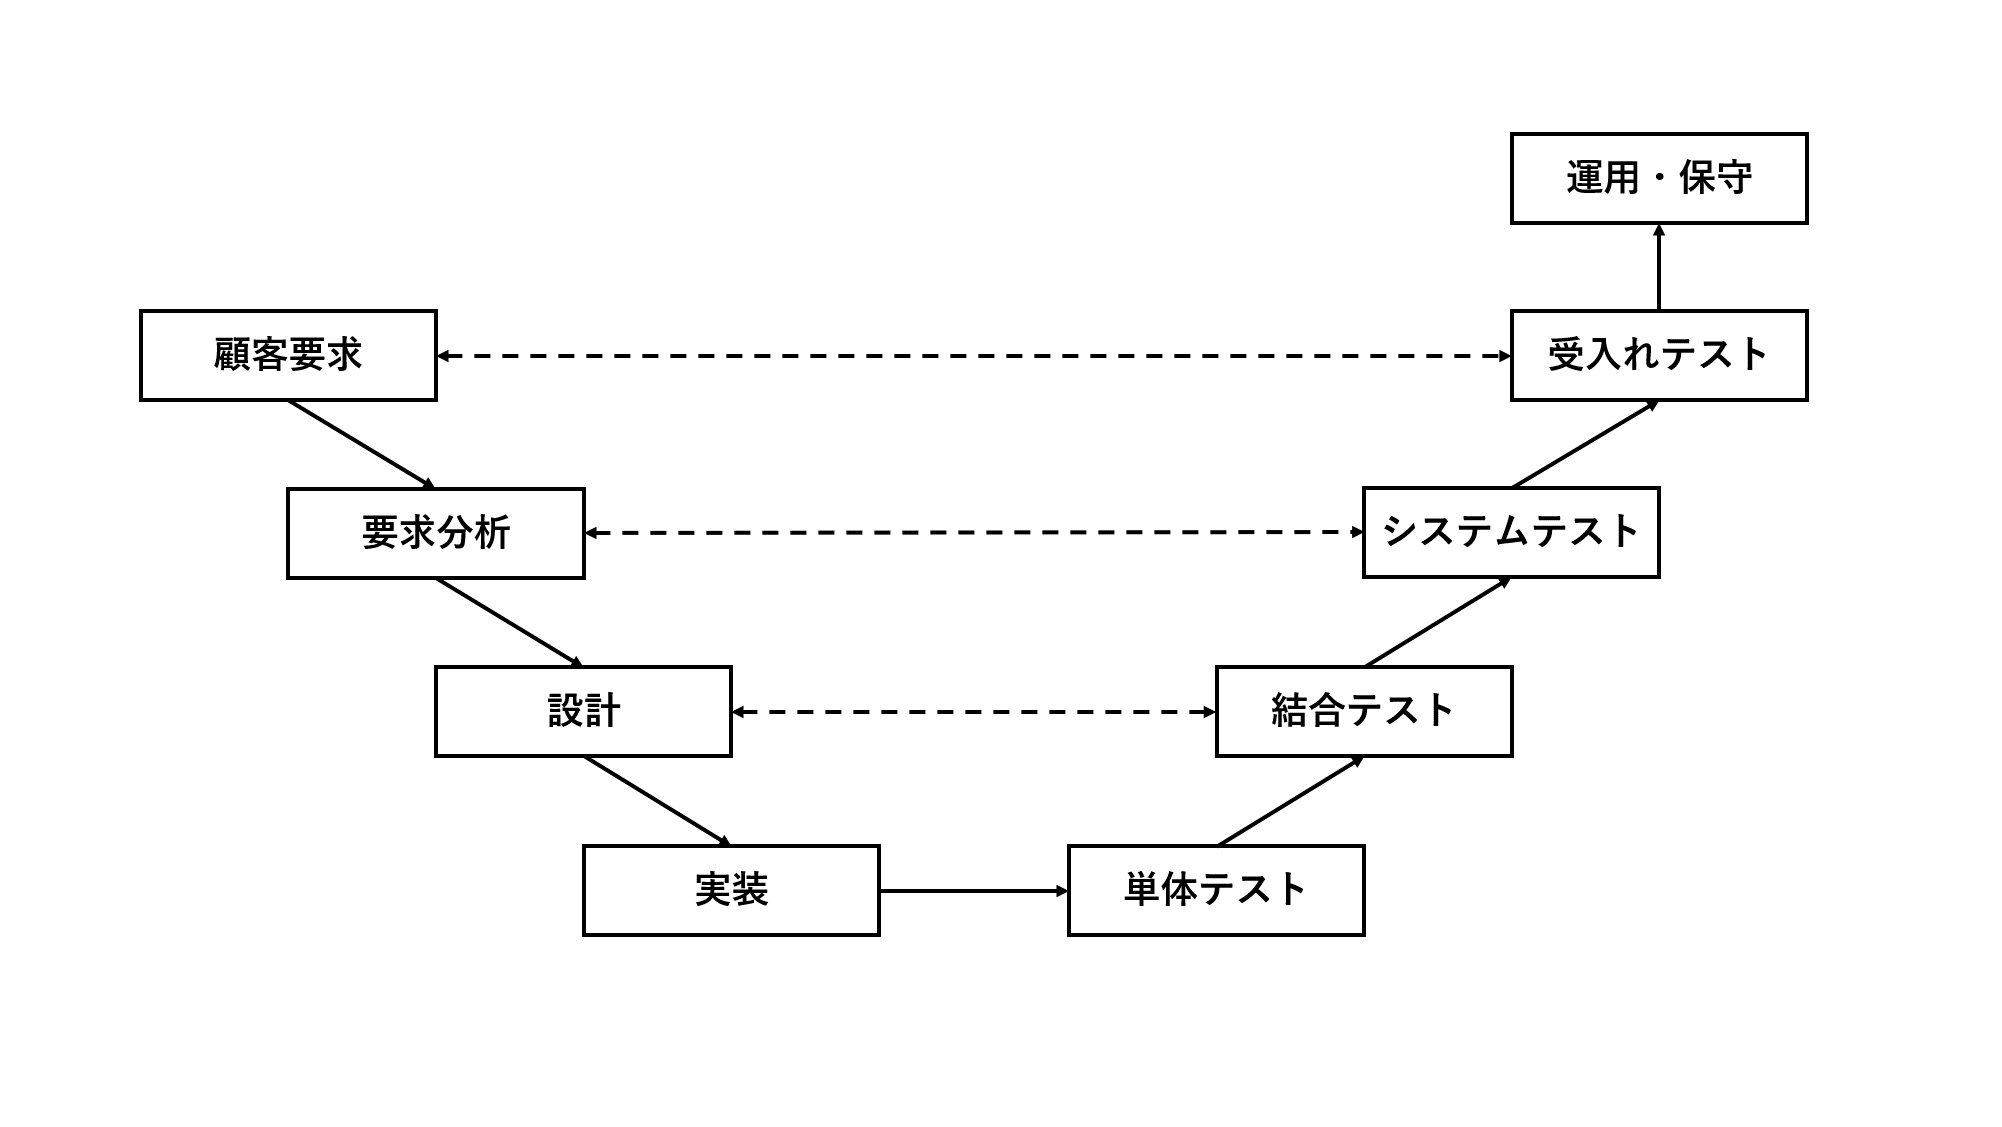
\includegraphics[width=12cm]{buiji.eps}
	\caption{V字モデル}
	\label{buiji}
\end{figure}


\subsection*{UML\cite{uml}}
UMLとは、統一モデリング言語(Unified Modeling Language)のことで、50以上の方法論やダイアグラム表記法のよさをできるだけ踏襲するように共通点を抽出すると同時に、オブジェクト指向でモデリングする際に必要な概念をすべて抽出し、それらを整理統合するような新たなモデル記述体系として考案されたものである。UMLを用いることで対象となる領域やシステムがどのような概念や要素から構成されているかという、構造的な側面のモデル化と、そうした概念や要素が時間経過の中でどのように相互作用して振る舞い、変化を行うかという動的な側面のモデル化の両方を、統一的でビジュアルな言語を使って行うことができる。そのため、組織やプロジェクト固有の慣習を捨象して世界共通の土台で議論できるようになり、計画やコンセプト作りから設計の詳細検討、実装やテストのための仕様定義といった様々な局面で普遍的に活用することができる。本研究でも、開発メンバー4人が1つのチームとして、共通認識を持って開発に取り組むため、要求分析・設計の工程でUML図を作成した。

\subsection*{ユースケース図\cite{uml}}
ユースケース図とは、システムがどのように機能すべきかという振る舞い(ユースケース)と、その外部環境(アクター)を表現するもので、システムの外部と内部との境界を明確にすることができる。ユースケース図を用いることで、エンドユーザの視点からシステムを見ることができ、エンドユーザや領域の専門家とのコミュニケーションが円滑になり、要求に対する相互の理解を保証することができるようになる。

\subsection*{アクティビティ図\cite{uml}}
 アクティビティ図とは、ひとまとまりの業務や処理の内容や流れを表すために、関連する複数の業務手順や処理ステップを順序だてて配置したもので、アクティビティ図によって、「企業全体や業務全体のモデルにおける一連のワークフロー」、「ユースケースごとに対応する処理フロー」、「あるオブジェクトの持つ1メソッドの内部のアルゴリズム」を記述することができる。

\subsection*{クラス図\cite{uml}}
クラス図とは、モデルの静的な構造を表現できる図であり、データ構造(属性リスト)と振る舞い(操作リスト)を持つクラスと、クラス間の静的な関係が表現できる。このクラス図が、UMLに代表されるオブジェクト指向分析設計における中心的な図となり、問題領域の構造や対象システムのアーキテクチャの静的な構成、システムの詳細設計、問題解決の発想の起点となる概念マップの構築といったことに広く用いることができる。

\subsection*{シーケンス図\cite{uml}}
シーケンス図とは、オブジェクト間のメッセージのやり取りを時系列に沿って並べて表現したもので、ユースケースを実現するのに必要なオブジェクトの集合と、その相互作用を明確に表現できる。ここでは、メッセージを時間順に1つずつ記述できるため、シナリオと対応させて具体的な内容を示す際に有用である。


%第3章 
\chapter{抗ノイズテストパターン生成法}
%第3章
本章ではまず、3.1節にて本研究で開発する「感染症予防サポートシステム」の概要を述べる。続いて3.2節ではユースケース図、ユースケース記述を用いて、システムの要求定義について述べる。3.3節ではアクティビティ図、クラス図を用いて、システムの基本設計について述べる。3.4節ではシーケンス図を用いてシステムの詳細設計について述べる。



%第4章
\chapter{実験結果・考察}
%第4章:実装・検証

本章ではV字開発モデルの開発プロセスに従い,実装および検証を行った結果を述べる.
4.1節では,各設計に基づいて行った実装について述べる.
4.2節ではそれぞれ詳細設計を単体テスト,基本設計を結合テスト,要求分析を総合テストによって検証した結果を示す.

%第5章
\chapter{あとがき}
%第5章
本章では、本システムに対する評価・考察を行い、今後の課題や将来性についても述べる。

まず3.1節に挙げた、本システムが果たすべき2つの大きな役割に対して評価する。3.1節において、本システムが果たすべき役割について、「感染症予防対策のルールを守ってもらうよう働きかける役割」、「感染症予防対策の基準を定める役割」の2つを挙げた。感染症予防対策のルールを守ってもらうよう働きかける役割については、室内環境に応じた換気要請の発出や、感染リスクのレベルの通知によって、換気や人数調整といった具体的なアクションを促すことが実現できていると考えられる。感染症予防対策の基準を定める役割については、利用者が感染症予防のためにとるべき、換気と部屋に滞在する人数の調整というアクションについて、感染症予防の観点から、部屋を安全な状態に保つため、具体的にその基準を定めることで、利用者自身が感染症予防のためにとるべきアクションを明確にすることが実現できていると考えられる。

また本システムでは、センサデバイスで取得したデータを随時データベースに記録しているほか、室内の滞在人数や警戒レベル、感染リスクといったデータも、センサデバイスからのデータ更新に伴って導き出されていることから、必要に応じてデータを保管しておくことで、システム外部で様々なデータの相関を調べることもできる。そのため、感染症予防対策の基準を定める役割に関しては、応用の余地があると考えられ、例えば以下のような応用の仕方が考えられる。

本システムでは、分析に活かせる多くのデータを導き出せるが、中でも設計の段階から分析に役立てられるデータとして着目していたのは、警戒レベルと感染リスクのデータである。既に述べたように、室内にある程度の人数が滞在していないと警戒レベルの導出は行われない。そのため警戒レベルの推移のデータは、その部屋が警戒レベルを導出できる条件下で利用されているとき、どの程度二酸化炭素濃度が高まりやすいかを確認でき、運用ルール改定の基準にできる。また、警戒レベルと感染リスクのデータをシステム内部で分析し、本システムでは固定的である、二酸化炭素濃度と警戒レベル、警戒レベルと滞在可能人数の関係を、部屋の警戒レベルと感染リスクの変動の仕方に応じて流動的に変化させると、よりその部屋にあった感染症予防対策を講じることが可能になると考えられる。

感染リスクのデータは、換気状況など、部屋の運用の仕方が適切であるかどうかを示しているため、部屋が感染症予防対策上、危険な状態で使用されていないかを確認できる。そのため学校やオフィス、公共施設などでの利用のケースを想定すると、時間帯ごとの感染症予防対策への取り組みの徹底度合いが、エビデンスとして残されることから、管理者側からの適切な指導が行えるほか、各部屋の責任者となる者が、感染症予防対策に、より注意して取り組むことができると考える。

本システムの設計時の着想では、利用環境ごとに異なる、床面積の広さ・空間の広さ、換気のしやすさや窓の位置と数、換気設備の有無、部屋利用者の活動の仕方などに柔軟に対応し、利用環境に合わせた感染症予防対策の基準を定め、利用者に感染症予防対策のルールを守ってもらうよう働きかけられることが本システムの特徴であった。実際に、本システムは4.2節の総合テストでの検証のように、様々なシナリオにあった感染症予防の働きかけが可能となることが考えられる。しかしながら、本システムでの感染症予防対策の基準の決め方では、換気のしやすさや、部屋の床面積の広さのわりに、ものが多く置かれているなどの理由から実際の空間が狭いというような部屋の特性が、そのまま二酸化炭素濃度の上昇の仕方に反映されることを前提としている部分があり、柔軟性に欠けていると考える。理想的な環境における本システムの実用性は確認されたものの、部屋ごとの特性を加味した感染症予防対策の基準を、実際の利用環境において適切に定めるためには、本システムでの室内環境の分析の仕方よりも複雑に、室内環境を分析する必要があるとも考えられ、部屋の特性自体をシステムの分析機能によって導き出すことができると、現在のシステムと比較し、よりその部屋の特性に適合した感染症予防対策の基準の設定を行うことができるため、更なる研究と改良の余地が大いに残されていると考える。



%--ここまで本文--


%謝辞
\newpage
\addcontentsline{toc}{chapter}{\protect\numberline{謝辞}{}}
\chapter*{謝辞}
%--ここから謝辞--
本研究を進めるにあたり,懇篤な御指導,御鞭撻を賜わりました本学高橋寛教授に深く御礼申し上げます.

本論文の作成に関し,詳細なるご検討,貴重な御教示を頂きました本学樋上喜信准教授に深く御礼申し上げます.

また,審査頂いた本学岡野大准教授ならびに宇戸寿幸准教授に深く御礼申し上げます.

最後に,多大な御協力と貴重な御助言を頂いた本学工学部情報工学科情報システム工学講座高橋研究室の諸氏に厚く御礼申し上げます.

%--ここまで謝辞--

%参考文献
\begin{thebibliography}{99}
%ここから参考文献

%--例--
\bibitem{Interconnect}
Bram Kruseman , Ananta K. Majihi , Wilmar Heuvalman , Jennifer Dworak“NIM-X : A Noise Index Model-Based X-Filling technique to Overcome the Power Supply Switching Noise Effects on Path Delay Test" IEEE Trans. on VLSI Test Symp. ,pp.809-813, May. 2012.
%ここまで参考文献

\end{thebibliography}
\end{document}
